\newpage
\section{Design and Implementation}
    \subsection{Input format}
    The input is the \textbf{Bayesian Interchange Format} (BIF) which is a file with .bif extension.
    In general, Four types of blocks are defined.\\
    \noindent \textbf{The Network Block:}\\
    A network block defines the name of the network and lists the properties. The example below specify the network block for the Asia Bayesian Network:
    \begin{lstlisting}
    network asia{
       property version 1.1;
       property author ..;
    }
    \end{lstlisting}
    
    \noindent \textbf{The Varable Block:}\\
    Variable blocks define the variables in a network. These blocks used
    to be called node blocks in the BNIF; it seems that variable conveys
    more of a statistical meaning while node just refers to a graphical
    concept. The example below is the bronc node from asia.bif
    \begin{lstlisting}
     variable bronc{
        type discrete [2] {yes, no};
     }
    \end{lstlisting}
    
    \noindent \textbf{Blocks for standard nodes}\\
    Standard nodes have to define the probabilities for each discrete parent instantiation. An example of a standard probability block is: 
    \begin{lstlisting}
     probability (dysp | bronc, either){
        (yes, yes) 0.9, 0.1;
        (no, yes) 0.7, 0.3;
        (yes, no) 0.8, 0.2;
        (no, no) 0.1, 0.9;
    }
    \end{lstlisting}
    
    \noindent \textbf{Probability blocks}:\\
    Probability blocks are another way to specify the (conditional) probability tables (CPTs). For these variables, and hence the topology of the network. The block indicates the variables of the probability distribution right after the keyword probability.
    \begin{lstlisting}
    probability (v_10_8 v_10_7 v_9_8){ 
	table 0.586357 0.667473 0.789088 0.466932 
	      0.413643 0.332527 0.210912 0.533068;
    }
    \end{lstlisting}
    A more detailed explanation of the BIF is explained here: \footnote{http://www.cs.washington.edu/dm/vfml/appendixes/bif.htm} \\
    
    \subsection{Output}
    The output of the program is the cnf file following the DIMACS format which is a widely accepted standard format for representing CNF clauses and it's also a format used by most of the model counters mentioned in section 3.3.\\
    \begin{itemize}
        \item A comment line starts with a \textit{c}
        \item A line p cnf var clauses specify the instance in CNF format, in which \textit{vars} is the number of variables used in the file and \textit{clauses} is the number of clauses in the CNF.
        \item Each CNF variable is denoted by a non\-zero number smaller than \textit{vars}, the negation of a variable is denoted by a negative number.
        \item Each clauses contains one or several CNF variables, 0 specifies the end of the clause.
    \end{itemize}
    
    Consider the following CNF:
    \begin{center}
        $x_{1} \vee x_{2} \vee \neg x_{3}$\\
        $x_{1} \vee x_{4} \vee x_{5}$\\
        $\neg x_{3} \vee \neg x_{4}$\\  
    \end{center}
    The clauses in DIMACS format\\
    \begin{center}
        \begin{lstlisting}
        c
        c A sample DIMAC file
        c
        p cnf 5 3
        1 2 -3 0
        1 4 5 0
        -3 -4 0
        \end{lstlisting}
    \end{center}
    
    \subsection{Fetching variables values from Bayesian Network}
    Pgmpy library does not support fetching CPT values using table indexing, the only way to fetch value is through specifying evidence and variables and query the value through Variable Elimination method. The Variable Elimination method is the bayesian inference method that is \textcolor{red}{Insert time complexety}. To solve the problem, I extended the pgmpy library to support fetching variable values without querying using Variable Elimination.\\
    
    The method get\_cpds returns a conditional probability distribution of the node, the returned type is defined as TabularCPD that contains the name of the node, cardinality, variables which are stores as a nested list, the list of evidences and their corresponding cardinalities. An example is given below:
    \begin{lstlisting}
        cpd = TabularCPD('dysp', 2, [[0.9, 0.7, 0.8, 0.1],
                                      [0.1, 0.3, 0.2, 0.9]],
                                     ['bronc', 'either'], [2, 2])
    \end{lstlisting}
    In our case for both bron and either, the evidence all equals to 2, the convention for the order is shown in figure \ref{fig:sample print table}. The list which store the values are the transpose of the matrix in BIF format.\\
    \begin{figure}
        \centering
        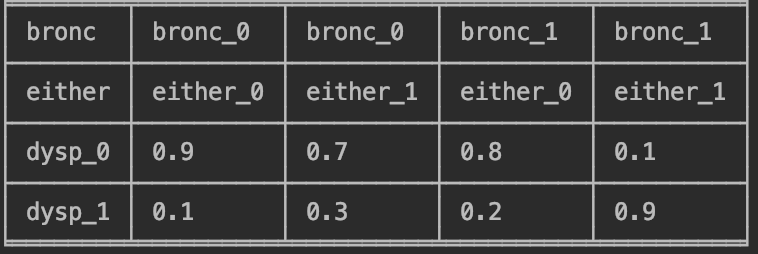
\includegraphics[width = 0.7\textwidth]{pic/printBayesnode.png}
        \caption{A sample printed CPT of a node dyps}
        \label{fig:sample print table}
    \end{figure}
    \subsection{Implementation of Full encoding}
    \textbf{Generating Indicator variables:}
    \begin{minted}
    [linenos]
    {python}
    def indicator(bn, var_dic, clauses, weights):
        for i in bn.nodes:
            cardinality <- bn.get_cardinality(i)
            # get variables
            for j in range(cadinality):
                name <- 'lambda_' + str(i)+ '_' + str(j)
                # append variable to variable dictionary
                # store the corresponding weights
                if name not in var_dic:
                    var_dic[name] = max(var_dic.values()) + 1
                    weights[name] = 1
            # get clauses:
        for i in bn.nodes:
            cardinality <- bn.get_cardinality(i)
            cl = [] # cl store each clause in the CNF, represented by a list of tuples
            for j in range(cardinality):
                variable <- fetch the corresponding variable from the dictionary
                cl.append((1, variable)) # 1 represent positive
            clauses.append(cl)
            
            for m in range(cardinality):
                for n in range(m + 1, cardinality):
                    var1, var2 <- fetch lambda_i_n, fetch lambda_i_m
                    cl = [(-1, var1), (-1, var, var2)]
                    clauses.append(cl)
    return clauses, var_dic, weights
    \end{minted}
    
    \textbf{Generating Parameter variables:}
    \begin{minted}
    [linenos]
    {python}
    def parameter_cl(bn, var_dic, clauses, weights):
        for i in bn.nodes:
            cardinality = i.get_cardinality()
            evidence = i.get_evidence()
            if no evidence:
                for j in cardinality:
                    name <- theta_ij
                    var_dic[name] <- max(var_dic.value()) + 1
                    weight[name] <- fetch weight
            else:
                ev_cardinality <- [ev.cardinality() for ev in i.evidence]
                evidence_lst <- generate evidence list()
                for j in cardinality:
                    for ev in evidence_lst:
                        name = 'theta_' + i + str(j) + '|' + ev
                        var_dic[name] <- max(var_dic.value()) + 1
                        weight[name] <- fetch weight
    return var_dic, clauses, weights

            
    \end{minted}
    
    Generating Parameter variables:
    Write files:
    Storing weights
    \subsection{Simplified Full encoding}
    \subsection{Implementation of Improved Encoding}
    \subsection{Implementation of Group Encoding}
        \subsubsection{Splitting the CPT}
        \subsubsection{QM algorithm and extension for multi-variate simplification}
